\documentclass{article}

\usepackage{graphicx}
\usepackage[hidelinks]{hyperref}
\usepackage{geometry}
\usepackage{amsmath}
\usepackage{listings}
\usepackage{wrapfig}
\usepackage{subcaption}
\usepackage{tikz}
\usetikzlibrary{positioning}

\geometry{
 a4paper,
 left=20mm,
 right=20mm,
 top=20mm,
 bottom=25mm,
}

\begin{document}

\begin{titlepage}
\begin{center}
\vspace*{1cm}
            
\Huge
\textbf{Project 3}
            
\vspace{1cm}

\Large
\text{Due: Friday, November 15, 2024}

\vspace{2cm}

\text{\texttt{Brian High}} \\
\text{\texttt{Thomas Hynes}} \\
\text{\texttt{Jeremy Middleman}} \\
\text{\texttt{Andrei Phelps}} \\
\text{\texttt{Wayne Rudnick}} \\

\vspace{2cm}

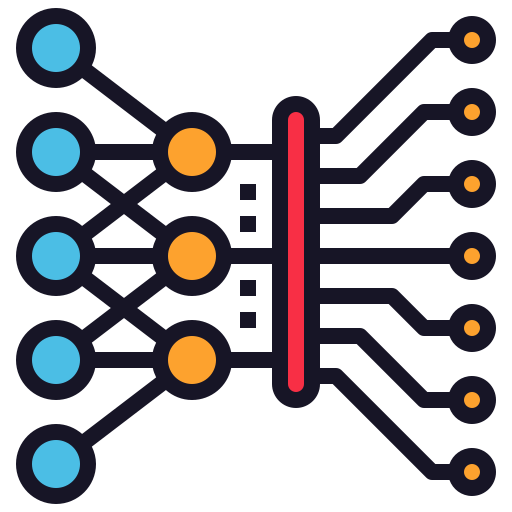
\includegraphics[scale=0.25]{figs/icon.png}\\[0.5cm]

\vspace{9cm}

\textbf{CS 491/591: Neural Networks} \\

\end{center}
\end{titlepage}

\newpage

\section{Code Execution}

To run the code, run: \\ \\
Notes: 

\section{Newton's Method}

\subsection{What is the Hessian?}
The Hessian matrix is a square matrix of second-order partial derivatives. Newton's method's goal is to make a 2nd order approximation and minimize it. The Hessian is how we calculate these 2nd order derivatives. For a function \( F \) with \( n \) parameters, the Hessian is an \( n \times n \) matrix, where each element \( H_{ij} \) represents the second-order partial derivative of \( F \) with respect to two parameters. In our case, the Hessian is \( n \times n \) matrix where n is the number of weights in the neural network. The hessian captures the curvature of the function along each individual parameter axis along with the interaction between pairs of parameters. This structure second-order optimization methods to work.

\subsection{Explain the update of the 1st and 2nd order deravtives}
To update each weight in a neural network, we use both first-order and second-order derivatives. The first-order derivative, or gradient, shows how much a small change in each weight affects the overall loss, and it’s calculated by backpropagation. The second-order derivative, found in the Hessian matrix, tells us how each gradient changes with respect to other weights, helping us understand the curve of the loss function. Using both gradients and the Hessian allows us to update weights more precisely by considering both the slope and curvature of the loss surface.

\subsection{Pseudo Code}

\begin{verbatim}
 Inputs:
   W: Weight matrix 
   grad: Gradient matrix 
   x: Input data point
   y: Target output


function computeHessian(W, grad, x, y):
    # Initialize Hessian list for each layer
    H = [zeros_like(layer) for layer in W]

    # Forward pass to compute activations
    activations = [x]  # Input is the first activation
    for layer_weights in W:
        x = activationFunction(dotProduct(layer_weights, x))
        activations.append(x)

    # Backward pass to compute Hessian
    for layer in reverse(W):
       for i and j in W
            # Compute second-order derivative
            activation_term = activationSecondDerivative(activations[layer]) * activations[layer-1][i]
            gradient_term = grad[layer][i][j]
            H[layer][i][j] = activation_term + gradient_term

    return H

\end{verbatim}

\subsection{Case 1: Computations}
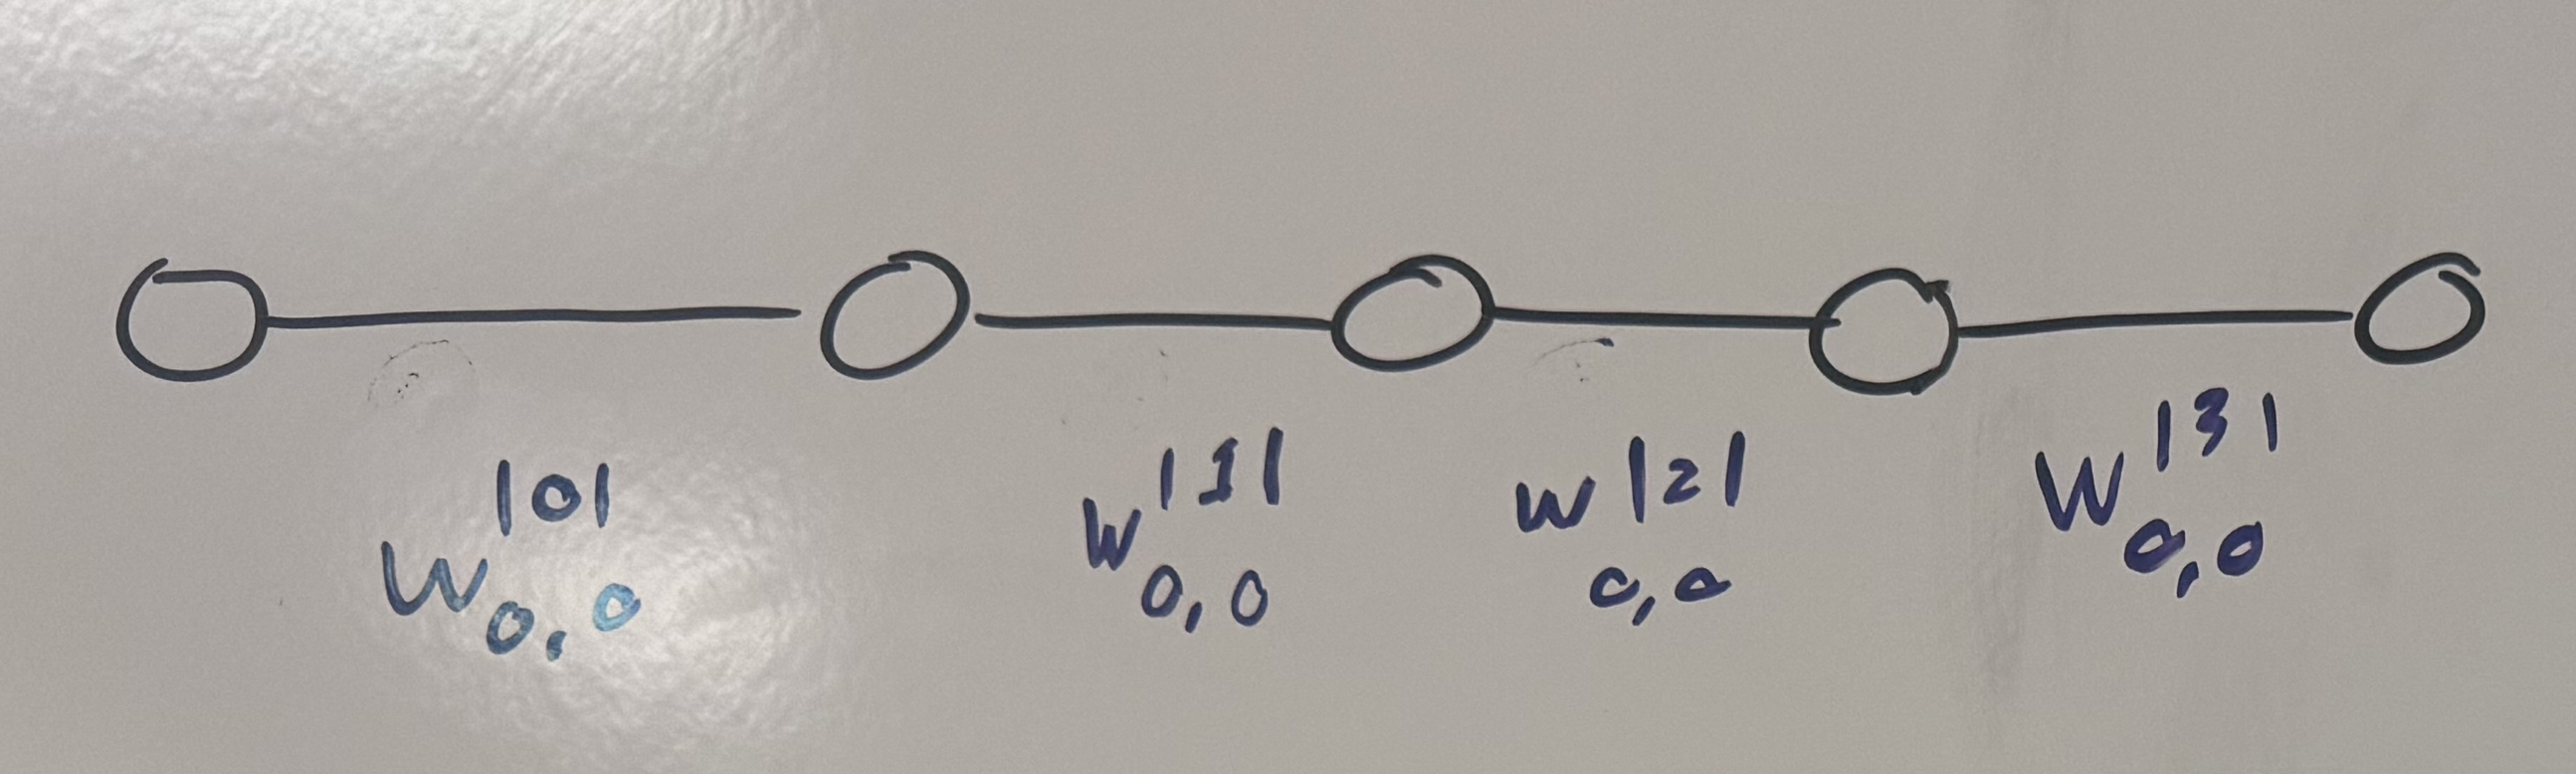
\includegraphics[scale=0.1]{../figs/Case 1.png} \\[0.5cm]

The following is an example how to compute the hessian on this nueral network using random values.

\subsubsection{Forward Pass}
The weights and biases are initialized randomly:
\[
x = 0.5, \quad W_1 = 0.8, \quad W_2 = -0.6, \quad W_3 = 0.4, \quad W_4 = 1.2
\]
\[
b_1 = 0.1, \quad b_2 = -0.2, \quad b_3 = 0.05, \quad b_4 = 0.3
\]
\paragraph{Compute layer activations:} Sigmoid activation function is used to compute the activation

\[
z_1 = W_1 \cdot x + b_1 = 0.5, \quad a_1 = \sigma(z_1) \approx 0.6225
\]
\[
z_2 = W_2 \cdot a_1 + b_2 \approx -0.5735, \quad a_2 = \sigma(z_2) \approx 0.3605
\]
\[
z_3 = W_3 \cdot a_2 + b_3 = 0.1942, \quad a_3 = \sigma(z_3) \approx 0.5484
\]
\[
z_4 = W_4 \cdot a_3 + b_4 = 0.9581, \quad \hat{y} = \sigma(z_4) \approx 0.7228
\]

\subsubsection{Back Propagation} Mean squared Error used for the loss function


\paragraph{Gradient of Loss with Respect to Output Layer}

\[
\frac{\partial L}{\partial \hat{y}} = \hat{y} - y = 0.7228 - 1 = -0.2772
\]

\paragraph{Error for Output Layer}
\[
\delta_4 = \frac{\partial L}{\partial \hat{y}} \cdot \sigma'(z_4)
\]

\[
\sigma'(z_4) = \hat{y} \cdot (1 - \hat{y}) = 0.7228 \cdot (1 - 0.7228) \approx 0.2002
\]

\[
\delta_4 = -0.2772 \cdot 0.2002 \approx -0.0555
\]

\paragraph{Gradients for \( W_4 \) and \( b_4 \)}
\[
\frac{\partial L}{\partial W_4} = \delta_4 \cdot a_3 = -0.0555 \cdot 0.5484 \approx -0.0304
\]
\[
\frac{\partial L}{\partial b_4} = \delta_4 \approx -0.0555
\]


\subsubsection{Repeat for layer 1-3}

\subsubsection{The resulting gradients for each weight and bias would look something like this:}
\[
\frac{\partial L}{\partial W_4} \approx -0.0304, \quad \frac{\partial L}{\partial b_4} \approx -0.0555
\]
\[
\frac{\partial L}{\partial W_3} \approx -0.0059, \quad \frac{\partial L}{\partial b_3} \approx -0.0165
\]
\[
\frac{\partial L}{\partial W_2} \approx -0.0009, \quad \frac{\partial L}{\partial b_2} \approx -0.0015
\]
\[
\frac{\partial L}{\partial W_1} \approx 0.0001, \quad \frac{\partial L}{\partial b_1} \approx 0.0002
\]

\subsubsection{Computing the Hessian}

The second-order gradients are the partial derivatives of each first-order gradient with respect to each weight. The Hessian element \( H_{ij} \) is given by:
\[
H_{ij} = \frac{\partial g_i}{\partial w_j} = \frac{\partial^2 L}{\partial w_i \partial w_j}
\]

Apply the chain rule to the gradients as you backpropagate through the network to get the hessian.

\\
For the diagonal elements, where \( i = j \), the second-order derivative is:
\[
H_{ii} = \frac{\partial^2 L}{\partial w_i^2}
\]
\\
For the off-diagonal elements, where \( i \neq j \), the second-order derivative is:
\[
H_{ij} = \frac{\partial^2 L}{\partial w_i \partial w_j}
\]

\paragraph{Resulting Hessians}

\[
H_1 = \begin{bmatrix}
\frac{\partial^2 L}{\partial (w_{1,1}^{[1]})^2} & \frac{\partial^2 L}{\partial w_{1,1}^{[1]} \partial w_{1,1}^{[2]}} & \frac{\partial^2 L}{\partial w_{1,1}^{[1]} \partial w_{1,1}^{[3]}} & \frac{\partial^2 L}{\partial w_{1,1}^{[1]} \partial w_{1,1}^{[4]}} \\
\frac{\partial^2 L}{\partial w_{1,1}^{[2]} \partial w_{1,1}^{[1]}} & \frac{\partial^2 L}{\partial (w_{1,1}^{[2]})^2} & \frac{\partial^2 L}{\partial w_{1,1}^{[2]} \partial w_{1,1}^{[3]}} & \frac{\partial^2 L}{\partial w_{1,1}^{[2]} \partial w_{1,1}^{[4]}} \\
\frac{\partial^2 L}{\partial w_{1,1}^{[3]} \partial w_{1,1}^{[1]}} & \frac{\partial^2 L}{\partial w_{1,1}^{[3]} \partial w_{1,1}^{[2]}} & \frac{\partial^2 L}{\partial (w_{1,1}^{[3]})^2} & \frac{\partial^2 L}{\partial w_{1,1}^{[3]} \partial w_{1,1}^{[4]}} \\
\frac{\partial^2 L}{\partial w_{1,1}^{[4]} \partial w_{1,1}^{[1]}} & \frac{\partial^2 L}{\partial w_{1,1}^{[4]} \partial w_{1,1}^{[2]}} & \frac{\partial^2 L}{\partial w_{1,1}^{[4]} \partial w_{1,1}^{[3]}} & \frac{\partial^2 L}{\partial (w_{1,1}^{[4]})^2}
\end{bmatrix}
\]

\subsection{Case 2:}

\includegraphics[scale=0.1]{../figs/Case 2.png} \\[0.5cm]

\subsubsection{Computations}
The steps for this more complex neural network would be exactly the same expect the hessian would end of being 12x12 and there would be far more calulations.In a network with more neurons per layer, like a Each weight affects multiple neurons, making the relationships between weights more complex. Calculating the Hessian requires tracking how pairs of weights interact across layers, which takes more steps than in a network with only one neuron per layer. This increased complexity means we need more calculations to fully understand how changes in each weight impact the overall network output.

\subsubsection{Resulting Hessian}
\[
H_2 = \begin{bmatrix}
\frac{\partial^2 L}{\partial (w_{1,1}^{[1]})^2} & \frac{\partial^2 L}{\partial w_{1,1}^{[1]} \partial w_{2,1}^{[1]}} & \cdots & \frac{\partial^2 L}{\partial w_{1,1}^{[1]} \partial w_{2,1}^{[4]}} \\
\frac{\partial^2 L}{\partial w_{2,1}^{[1]} \partial w_{1,1}^{[1]}} & \frac{\partial^2 L}{\partial (w_{2,1}^{[1]})^2} & \cdots & \frac{\partial^2 L}{\partial w_{2,1}^{[1]} \partial w_{2,1}^{[4]}} \\
\vdots & \vdots & \ddots & \vdots \\
\frac{\partial^2 L}{\partial w_{2,1}^{[4]} \partial w_{1,1}^{[1]}} & \frac{\partial^2 L}{\partial w_{2,1}^{[4]} \partial w_{2,1}^{[1]}} & \cdots & \frac{\partial^2 L}{\partial (w_{2,1}^{[4]})^2}
\end{bmatrix}
\]
\section{Experiments and Results}

\subsection{Steepest Gradient Descent Method}

\subsubsection{Experiment with 100 Epochs}
The initial experiment involved training the neural network using the Steepest Gradient Descent (SGD) method for 100 epochs. The distribution of correct versus incorrect classifications for each digit is illustrated in Figure~\ref{fig:gd_100ep}. The network achieved an overall accuracy of 86.53\%, performing well across most digits, particularly those with less variability. Digits such as 2, 3, and 8 showed higher misclassification rates, suggesting challenges in their complex features.

\begin{figure}[h!]
    \centering
    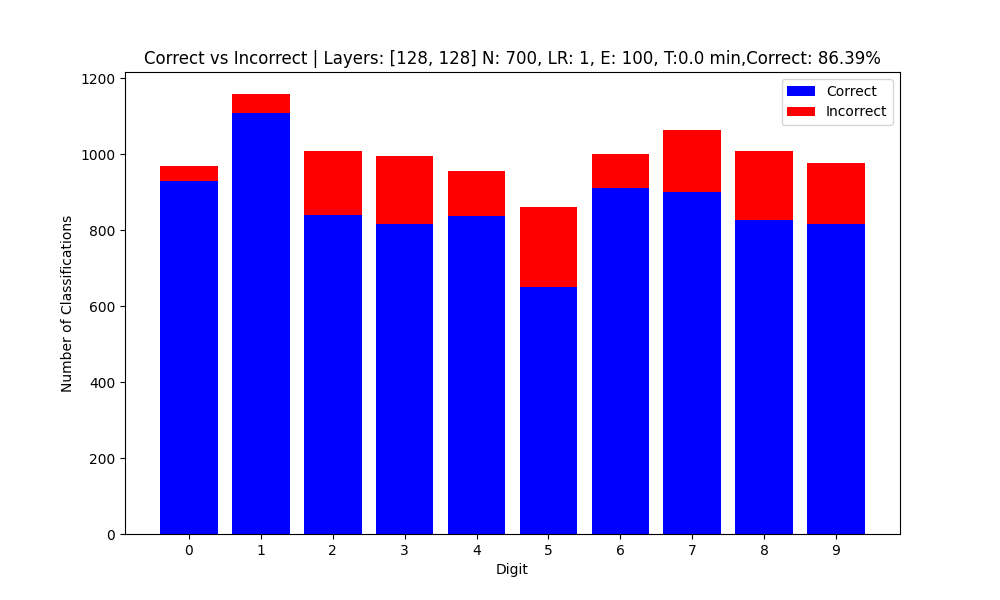
\includegraphics[scale=0.5]{../figs/gd_100ep.png}
    \caption{Gradient Descent with 100 Epochs}
    \label{fig:gd_100ep}
\end{figure}

\subsubsection{Experiment with 1,000 Epochs}
When the training duration was increased to 1,000 epochs, the accuracy improved slightly to 86.39\%. As depicted in Figure~\ref{fig:gd_1000ep}, this modest gain indicates diminishing returns from extended training under the existing network parameters.

\begin{figure}[h!]
    \centering
    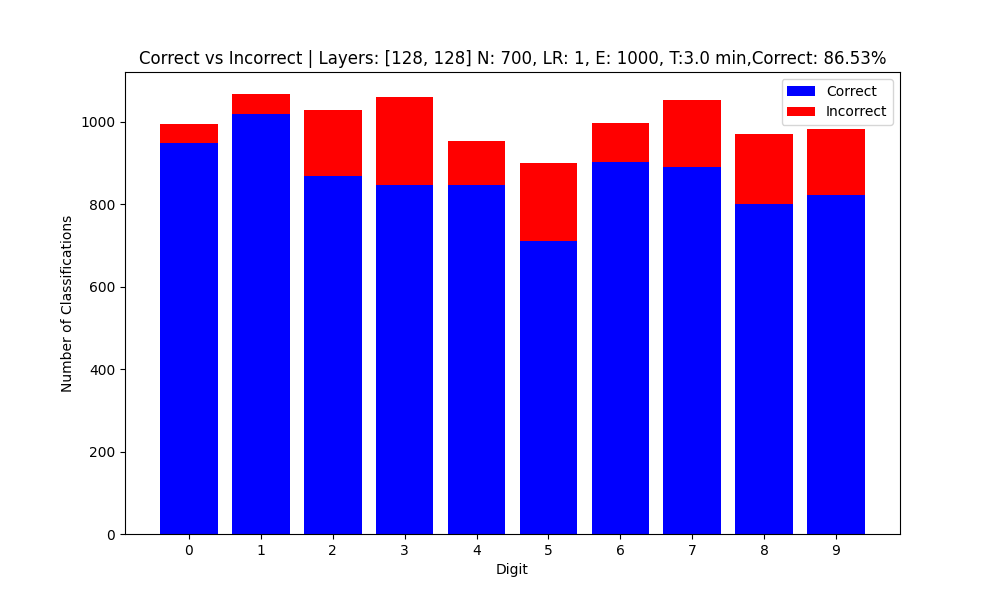
\includegraphics[scale=0.5]{../figs/gd_1000ep.png}
    \caption{Gradient Descent with 1,000 Epochs}
    \label{fig:gd_1000ep}
\end{figure}

\subsection{Nesterov Momentum-Based Learning}

\subsubsection{Experiment with 100 Epochs}
Utilizing Nesterov momentum for the initial 100 epochs, the network logged a classification accuracy of 86.05\%, as shown in Figure~\ref{fig:Nes_100ep}. This result underlines the effectiveness of Nesterov momentum in handling early training phases, albeit with some challenges in accurately classifying more complex digits.

\begin{figure}[h!]
    \centering
    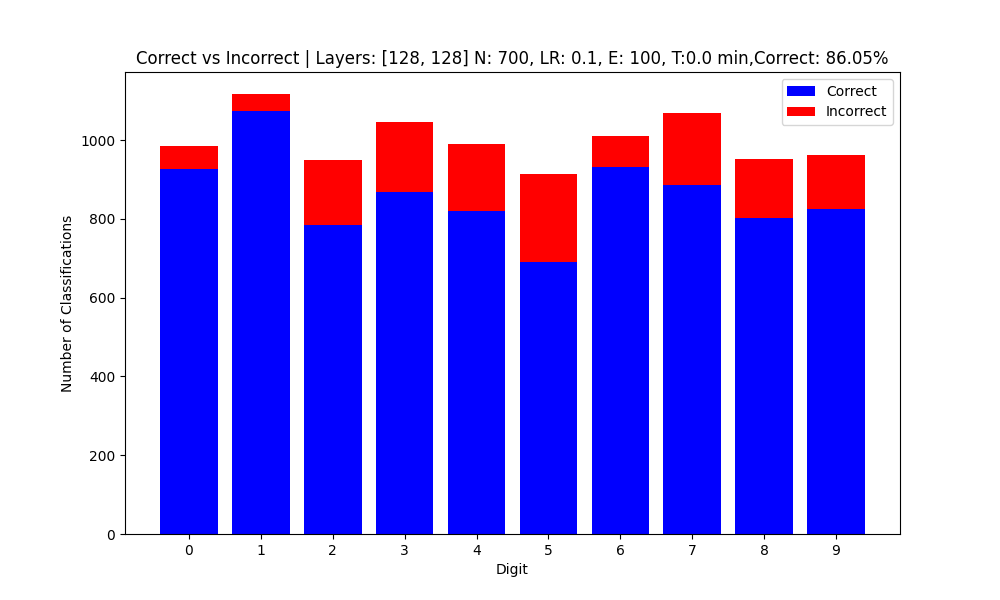
\includegraphics[scale=0.5]{../figs/Nes_100ep.png}
    \caption{Nesterov Momentum with 100 Epochs}
    \label{fig:Nes_100ep}
\end{figure}

\subsubsection{Experiment with 1,000 Epochs}
Increasing the epoch count to 1,000 raised the accuracy to 86.69\%. Figure~\ref{fig:Nes_1000ep} highlights incremental accuracy improvements, reinforcing the value of extended training periods with Nesterov momentum for gradual performance enhancements.

\begin{figure}[h!]
    \centering
    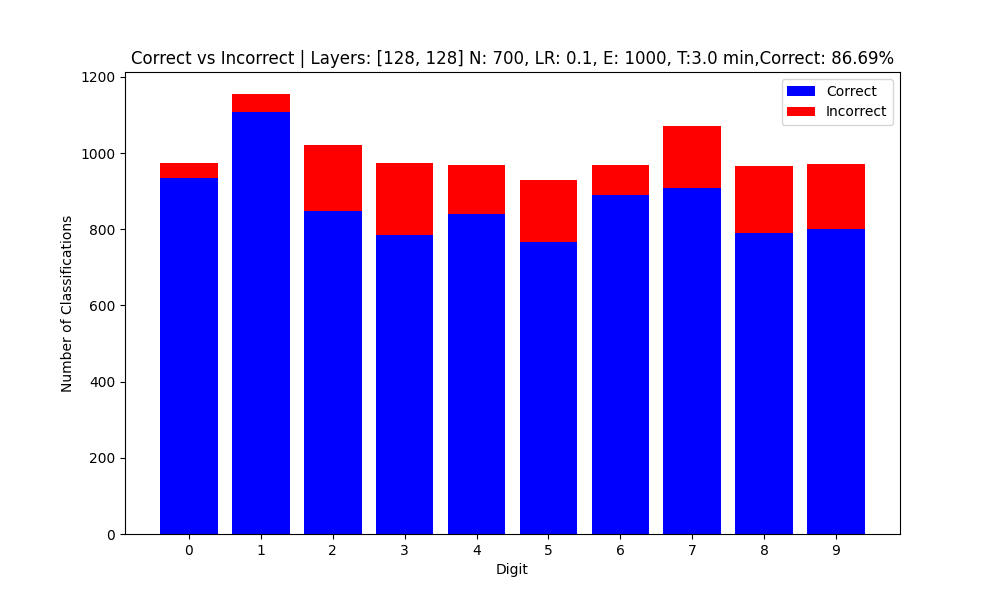
\includegraphics[scale=0.5]{../figs/Nes_1000ep.png}
    \caption{Nesterov Momentum with 1,000 Epochs}
    \label{fig:Nes_1000ep}
\end{figure}

\subsection{Adam's Method}

\subsubsection{Experiment with 100 Epochs}
Adam's method demonstrated rapid attainment of higher accuracy, reaching 87.17\% in just 100 epochs, as detailed in Figure~\ref{fig:Adam_100ep}. This efficiency underscores Adam's robustness in navigating complex datasets efficiently.

\begin{figure}[h!]
    \centering
    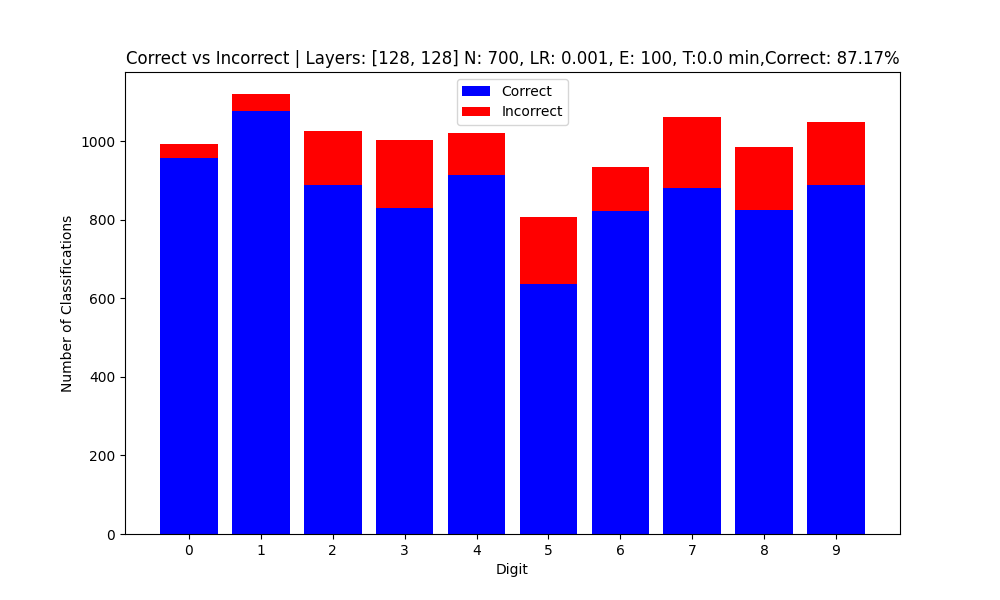
\includegraphics[scale=0.5]{../figs/Adam_100ep.png}
    \caption{Adam's Method with 100 Epochs}
    \label{fig:Adam_100ep}
\end{figure}

\subsubsection{Experiment with 1,000 Epochs}
Further training to 1,000 epochs marginally improved the accuracy to 87.74\%, with Figure~\ref{fig:Adam_1000ep} showing that while Adam is highly effective in optimizing learning, there is a plateau in performance gains with additional training.

\begin{figure}[h!]
    \centering
    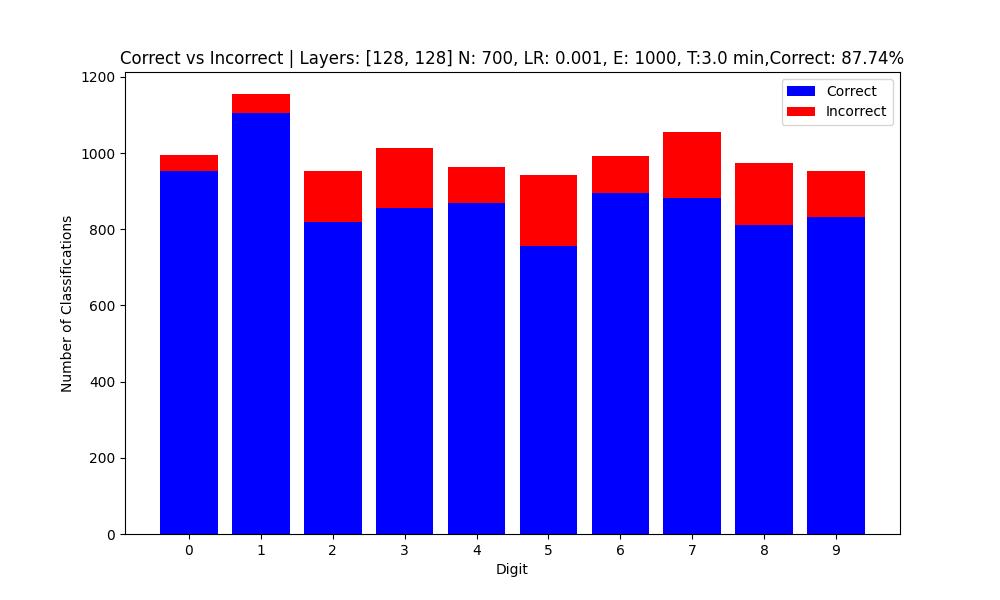
\includegraphics[scale=0.5]{../figs/Adam_1000ep.png}
    \caption{Adam's Method with 1,000 Epochs}
    \label{fig:Adam_1000ep}
\end{figure}

\newpage

\subsection{All Methods Compared}
The results offer a detailed comparison between three prominent learning methods—Steepest Gradient Descent (SGD), Nesterov Momentum, and Adam's Method—applied to a digit recognition task. The evaluation metrics include training time, prediction accuracy, and learning rate effectiveness. The figure below illustrates the performance comparison.

\begin{figure}[h!]
    \centering
    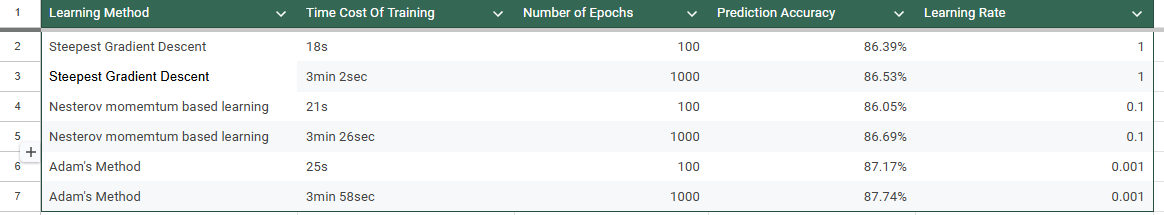
\includegraphics[scale=0.5]{../figs/LearningMethodsCompared.png}
    \caption{Comparison of Learning Methods}
    \label{fig:Comparison}
\end{figure}

\subsubsection{Steepest Gradient Descent}
SGD demonstrates its strengths in shorter training scenarios, achieving an accuracy of 86.39\% after 100 epochs with a training time of 18 seconds. Extending training to 1000 epochs marginally improved the accuracy to 86.53\%, but the time increased significantly to 3 minutes and 2 seconds. The aggressive learning rate of 1 enables fast convergence but often limits performance enhancement over longer training due to potential overshooting near optimal solutions.

\subsubsection{Nesterov Momentum}
In initial training phases, Nesterov Momentum recorded a slightly lower accuracy of 86.05\% after 100 epochs, taking 21 seconds. Its performance excels over longer periods, achieving 86.69\% accuracy after 1000 epochs, which takes 3 minutes and 26 seconds. The moderate learning rate of 0.1 enhances stability and optimization, effectively refining weights through its advanced momentum technique. This method balances training speed with precision and shows a notable improvement in sustained training epochs, though at a slight computational cost.

\subsubsection{Adam's Method}
Adam's Method shows superior results in both short and extended training periods. It reached 87.17\% accuracy within just 100 epochs, taking 25 seconds, and improved to 87.74\% over 1000 epochs, requiring 3 minutes and 58 seconds. Adam's lower learning rate of 0.001, combined with its adaptive gradient updates, supports excellent optimization capabilities, especially in complex loss landscapes. While Adam incurs the highest computational costs among the methods due to its management of momentum and variance terms, its effectiveness in achieving high accuracy makes it preferable for precision-critical tasks. \\ \\
\textbf{Summary:} Adam's Method emerges as the optimal choice for scenarios where accuracy is critical, albeit at the expense of higher computational demands. Nesterov Momentum provides a balanced approach with better performance over prolonged training, suitable for applications where gradual improvement is necessary. SGD, being the quickest, is ideal for rapid prototyping and scenarios where computational resources are limited. Choosing the right method hinges on specific project needs, considering trade-offs between accuracy, training speed, and computational resources.

\section{Individual Contributions}

\subsection*{Brian High}
\begin{itemize}
    \item[1)] Started programming Newtons Method
    \item[2)] Wrote the report on Newtons Method
\end{itemize}

\subsection*{Thomas Hynes}
\begin{itemize}
    \item[1)] 
\end{itemize}

\subsection*{Jeremy Middleman}
\begin{itemize}
    \item[1)] 
\end{itemize}

\subsection*{Andrei Phelps}
\begin{itemize}
    \item[1)] Implemented the Xavier initialization function.
    \item[2)] Collaborated on integrating the Nesterov Momentum-Based optimization technique.
    \item[3)] Assisted in conducting and analyzing the experimental results.
    \item[4)] Helped review and finalize report.
\end{itemize}

\subsection*{Wayne Rudnick}
\begin{itemize}
    \item[1)] Integrated the learning methods in with the testing system.
    \item[2)] Ran the Digits tests with the various learning methods
     \item[3)] Reported on the results and made the spreadsheet comparing the num epochs, accuracy, etc.
\end{itemize}

\end{document}
